\documentclass[makeidx, a4paper, 14pt]{extarticle}
\usepackage{makeidx}
\usepackage[top=1in, bottom=1.25in, left=1.25in, right=1.25in]{geometry}

% Enable cyrillic support
\usepackage[T1,T2A]{fontenc}
\usepackage[utf8]{inputenc}
\usepackage[main=russian,english]{babel}

% Images
\usepackage{graphicx}
\usepackage{float}

% Hyper text
\usepackage{hyperref}

% Math
\usepackage{amssymb, amsthm, amsmath, euscript}

% Figures
\usepackage{graphicx}
\usepackage{subfigure}

% Title page
\usepackage{fancyhdr}

% Section titles.
\usepackage{titlesec}

% Sections
\newcommand{\sectionbreak}{\clearpage}

% Symbols
\newcommand{\R}{\mathbb{R}}
\newcommand{\N}{\mathbb{N}}
\newcommand{\Z}{\mathbb{Z}}

% Define blocks.
\newtheorem{definition}{Определение}

% Disable links border
\hypersetup{hidelinks}

\graphicspath{ {./images/} }

\begin{document}

\begin{titlepage}
    \thispagestyle{fancy}
    \renewcommand{\headrulewidth}{0pt}
    \begin{center}
        МОСКОВСКИЙ ГОСУДАРСТВЕННЫЙ УНИВЕРСИТЕТ \\
        имени М.В. ЛОМОНОСОВА
        \medskip
        ФИЛИАЛ В ГОРОДЕ ТАШКЕНТЕ

        \bigskip
        \bigskip

        ФАКУЛЬТЕТ ПРИКЛАДНОЙ МАТЕМАТИКИ И ИНФОРМАТИКИ
        \medskip
        КАФЕДРА ПРИКЛАДНОЙ МАТЕМАТИКИ И ИНФОРМАТИКИ

        \bigskip
        \hrule
        \bigskip

        \large{Ванесян Роман Грачикович}

        \bigskip
        \bigskip

        \textbf{ВЫПУСКНАЯ КВАЛИФИКАЦИОННАЯ РАБОТА}

        \bigskip
        \bigskip

        \textbf{«Оптическое распознавание схем из функциональных элементов»}

        \bigskip
        \bigskip
        \bigskip
        \bigskip
        \bigskip
        \bigskip

        \begin{small}
            \begin{flushleft}
              Научный руководитель, \\
              к.ф.-м.н. \underline{\hspace{10cm}} Шуткин Ю.С.
            \end{flushleft}

            \smallskip

            \begin{flushright}
              «\underline{\hspace{1cm}}» \underline{\hspace{3.5cm}} 2020 г.
            \end{flushright}
        \end{small}

        \cfoot{ТАШКЕНТ - 2020}
    \end{center}
\end{titlepage}

\newpage

\section*{Аннотация}
В данной работе рассматривается проблема распознавания графического изображения схемы из функциональных элементов. Схема из функциональных элементов --- это
ориентированный граф с вершинами специального вида и ребрами, --- жордановыми дугами. Результатом данной работы является прототип программы,
которая показывает эффективность подхода описанного в данной работе. Результатом данной программы может быть как текстовая запись формулы
представленной данной схемой из функциональных элементов, так и сгенерированный код на языке DOT \cite{dot_lang}.

\tableofcontents

\section{Введение}
Зачастую при проектировании схем из функциональных элементов черновой вариант строится на листке бумаги с помощью обыкновенной ручки, либо карандаша.
Построенную схему далее хотелось бы моделировать с помощью программ специально предназначенных для этого. Появляется проблема, --- как перевести уже
имеющуюся схему в формат, с которым можно работать в данных программах? В данной работе представлен алгоритм позволяющий распознавать графические изображения
схем из функциональных элементов и по полученным данным генерировать код, который далее может быть интерпретирован с помощью таких специальных программ. \\
Вообще говоря, схема из функциональных элементов строится по заданной логической формуле. Данный процесс называется \emph{синтезом} схемы из функциональных элементов.
При синтезе схем для достаточно сложных формул может возникнуть проблема некорректного ее построения. Применяя подход описанный в данной работе, можно так же построить
алгоритм для валидации полученных схем в ходе синтеза.

\section{Постановка задачи}
Пусть задано некоторое множество булевых функций \[{B = {f_1(x_1, \dots, x_{n_1}), \dots, f_s(x_1, \dots, x_{n_s})}}, \]
где $n_1, \dots, n_s \ge 0$. \\ Будем называть данное множество $B$ \emph{базисом}.

\begin{definition}
    Схемой из функциональных элементов (СФЭ) над стандартным базисом ${B = \{x_1 \wedge x_2, x_1 \vee x_2, \neg{x_1}\}}$
    будем называть ориентированный граф без циклов ${G=(V, E)}$, для которого выполняются следующие условия:
    \begin{itemize}
        \item Каждая вершина $v \in V$ имеет полустепень захода $d(v)$, не превосходящую двух, то есть ${d(v) \le 2}$;
        \item Каждая вершина $v \in V$ с полустепенью захода, равной 0, называется входной (или входом схемы) и ей приписывается некоторая булева переменная $x_i$;
        \item Существует ровно одна вершина с полустепенью захода, равной 1 и приписанной меткой $F$, называемая выходом СФЭ;
        \item Все другие вершины называются внутренними вершинами схемы;
        \item Каждой внутренней вершине $v \in V$ с полустепенью захода, равной 1 приписывается (функциональный) элемент отрицания ($\neg$);
        \item Каждой внутренней вершине $v \in V$ с полустепенью захода, равной 2 приписывается либо (функциональный) элемент конъюнкции ($\vee$),
        либо (функциональный) элемент дизъюнкции ($\wedge$).
    \end{itemize}
\end{definition}

Стоит отметить, что существуют СФЭ с базисами отличными от приведенного. Однако, для упрощения изложения в данной работе мы будем рассматривать СФЭ
только со стандартным базисом.

При изображении схемы из функциональных элементов входы будем обозначать окружностями, внутри которых записаны входные переменные $x_i$.
Вершины являющиеся операциями, --- треугольниками, внутри которых записаны обозначения соответствующих функций.
А выход СФЭ будем помечать прямоугольником, внутри которого записана метка $F$. Выходы функций будем отмечать
выходными ребрами --- жордановыми дугами.

\begin{figure}[!h]
    \centering
    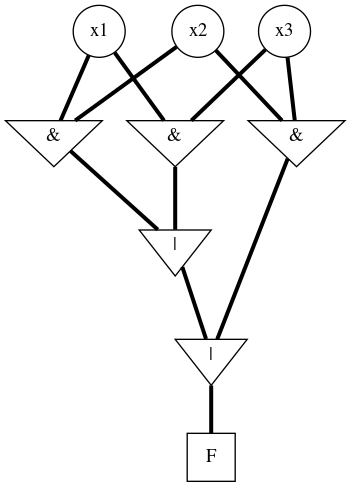
\includegraphics[scale=0.75]{img4.png}
    \caption{Пример изображения схемы из функциональных элементов.}
\end{figure}

\begin{definition}
    Цифровым изображением будем называть конечное множество ${I = \{p_i \mid p_i \in C\}}$ на плоскости,
    где $C$ --- либо конечное множество кортежей арности $3$, где каждый элемент имеет значение от $0$ до $255$,
    то есть: \[ {C=\{p_i \mid p_i=({x_{i_1}}, {x_{i_2}}, {x_{i_3}}), 0 \leq {x_{i_j}} \leq 255, j=\overline{1,3}\}}, \]
    в таком случае будем называть цифровое изображение трехканальным цифровым изображение;
    либо конечное множество элементов, значение которых варьируется от $0$ до $255$, то есть: \[ {C=\{p_i \mid p_i \in \Z, 0 \leq p_i \leq 255\}}, \]
    в таком случае будем называть цифровое изображение одноканальным цифровым изображение (полутоновое изображение). Элементы данного множества $p_i$ будем называть пикселями.
\end{definition}

\begin{definition}
    Одноканальное цифровое изображение, для которого множество $C$ определено как ${\{0, 1\}}$ будем называть бинарным цифровым изображением (бинарным изображением).
\end{definition}

На вход программе подается цифровое изображение со схемой из функциональных элементов. Выходом программы является либо текстовая
запись формулы представленной СФЭ, либо сгенерированный код на языке DOT \cite{dot_lang}. Полученный код может быть использован для дальнейшего моделирования СФЭ с помощью специальных программ, либо интерпретирован в более ``удобное''
графическое представление СФЭ, например, с помощью программы Graphviz \cite{graphviz}.

\section{Оптическое распознавание схем из функциональных элементов}

Оптическое распознавание СФЭ будем проводить в 4 этапа: предварительная обработка цифрового изображения, сегментация, распознавание, постобработка данных.

\subsection{Предварительная обработка данных}

Как и в любой задаче распознавания визуальных образов этап предварительной обработки направлен на разделение пикселей на два класса: ``фоновые'' пиксели и ``полезные'' пиксели
(пиксели образующие исследуемый объект). \\

Пусть на вход программе было подано трехканальное цифровое изображение. Применяя, к примеру, следующую функцию \cite{grayscale_luma}:
\[ f(x_1, x_2, x_3) = \lfloor 0.299 * x_1 + 0.587 * x_2 + 0.114 * x_3 \rfloor \] к каждому пикселю
$p_i=({x_{i_1}}, {x_{i_2}}, {x_{i_3}})$ преобразуем исходное трехканальное цифровое изображение в одноканальное цифровое изображение (полутоновое изображение).
Далее, к полученному полутоновому изображению, применяя алгоритм бинаризации с использованием метода Оцу \cite{otsu79} для нахождения оптимального порога бинаризации за счет
минимизации внутриклассовой дисперсии, получаем бинарное изображение.

\begin{figure}[H]
    \centering
    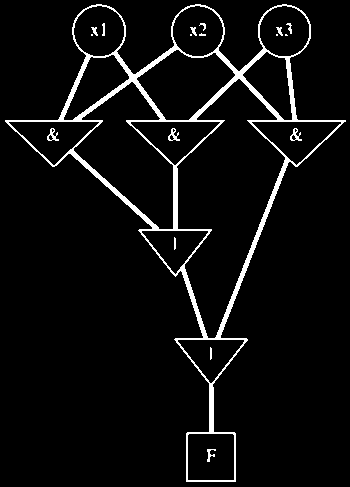
\includegraphics[scale=0.75]{img4_binary.png}
    \caption{Пример применения алгоритма бинаризации.}
\end{figure}

\subsection{Сегментация}

Входными данными для процесса сегментации является бинаризованное изображение.

Положим $D$ --- множество всех пикселей бинаризованного изображения.

\begin{definition}
    Множество пикселей ${V = \{p_i \mid p_i \in D\}}$ будем считать вершиной, если для него выполняются следующие 3 условия:
    \begin{enumerate}
        \item Пусть ${F \subset V}$. Множество ${H = \{p_i \mid p_i \in F, p_i=1\}}$ образует одну из следующих фигур: треугольник, окружность, либо прямоугольник.
        \item Пусть ${G = F \setminus H}$. Существует такое подмножество \\
              ${M=\{p_i \mid p_i \in G, p_i=1\}}$ --- метка вершины.
        \item Никакие две рядом лежащие вершины не расположены так,
              что пересечение минимальных описывающих прямоугольников,
              содержащих соответствующие вершины есть множество не пустое, то есть: \\
              ${\forall V_i, V_j, \quad V_i \neq V_j, i \neq j: P(V_i) \cap P(V_j) = \varnothing}$.
    \end{enumerate}
\end{definition}

Исходя из определения вершин, мы можем построить алгоритм для нахождения таковых в бинарном изображении.
Применим алгоритм для нахождения замкнутых контуров \cite{suzuki85} к данному бинарному изображению.
Выходом алгоритма является множество $A$ с занумерованными элементами --- последовательности наборов координат, однозначно
задающими фигуры образованные различными замкнутыми контурами. Стоит отметить, что для проверки \textbf{условий 2, 3} нас интересуют минимальные прямоугольники
коллинеарные осям (в английской литературе axis-aligned minimum bounding box). Любой прямоугольник может быть задан
двумя точками: левой верхней и правой нижней точками (относительно начала координат). То есть, положим $p_{1}$ - левая верхняя,
а $p_2$ - правая нижняя точки, тогда: \[ \{ p_1=(min(x), max(y)), p_2=(max(x), min(y)) \}, \]
где минимум и максимум соответствующих координат берутся по всем наборам задающим описываемую фигуру.
Применяя данный алгоритм к каждому элементу множества $A$ мы получим множество минимальных описывающих прямоугольники. \\

\begin{figure}[H]
    \centering
    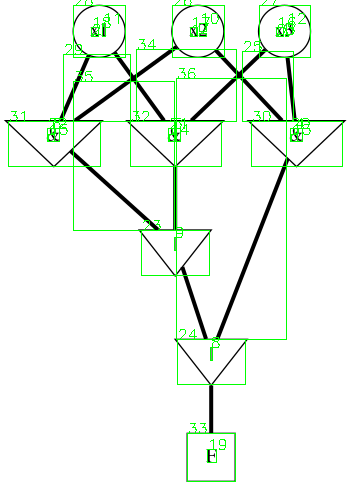
\includegraphics[scale=0.75]{img4_contours.png}
    \caption{Пример результата работы алгоритма построения минимальных описывающих прямоугольников.}
\end{figure}

\textbf{Проверим условие 1}.
Для проверки условия 1, для каждого описывающего минимального прямоугольника пометим все пиксели входящие во внутренность описываемой фигуры цветом $1$ (то есть присвоим им значение равное $1$),
все остальные пиксели прямоугольника - цветом $0$. Размер каждого такого изображение есть ${w \times h}$, где $w$ --- ширина, а $h$ --- высота.
Построим 3 бинарных изображения размера $w \times h$ с рисунками: окружности с радиусом ${r = \frac{min(w, h)}{2}}$ и центром в точке ${(\frac{w}{2}, \frac{h}{2})}$, прямоугольника c шириной $w$ и высотой $h$,
треугольника заданного координатами ${\{(0, h), (\frac{w}{2}, 0), (w, h)\}}$. Аналогично фоновые пиксели пометим цветом $0$, а внутренность с контуром каждой из фигур в цвет $1$.

Очевидно, что полученные изображения могут быть заданы матрицами размерности ${w \times h}$.

Положим

\[
    \delta(A, B) = \sum_{i=1}^{h}\sum_{j=1}^{w} a_{ij} \oplus_2 b_{ij}, \quad a_{ij} \in A, b_{ij} \in B
\]

Пусть матрица $A$ задает изображение вершины. Тогда будем считать, что на матрице $A$ изображена одна из трех фигур (окружность, прямоугольник, треугольник),
если сумма $\delta(A, B)$ - минимальна и не превышает некоторого заданного числа $k \in \R$.

\begin{figure}[H]
    \centering
    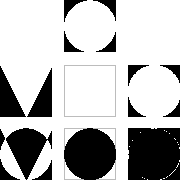
\includegraphics[scale=4]{shape_diff.png}
    \caption{Пример результата работы алгоритма проверки условия 1.}
\end{figure}

\textbf{Проверим условие 2}.
Положим \[
    c(p_{11}, p_{12}, p_{21}, p_{22}) = \begin{cases}
        1, &(p_{11} \le p_{21} \le p_{22} \le p_{12}) \\
        0, &\textrm{otherwise}
    \end{cases},
\]
где ${(p_{11}, p_{12})}$ и ${(p_{21}, p_{22})}$ пары левой-верхней и правой-нижней точек, задающих соответствующие прямоугольники.
Правило порядка для точек задано покоординатно.

Применяя попарно указанное правило к элементам множества минимальных описывающих прямоугольников, однозначно проверим условие 2.
То есть, если найдется такой минимальный описывающий прямоугольник не содержащий никаких других прямоугольников, то исключим фигуру вписанную в данный прямоугольник
из множества вершин. \\

\textbf{Проверим условие 3}.
Положим \[
    s(p_{11}, p_{12}, p_{21}, p_{22}) = \begin{cases}
        1, &(p_{11} \leq p_{21} \leq p_{12}) \wedge (p_{11} \le p_{22} \le p_{12}) \\
        0, &\textrm{otherwise}
    \end{cases},
\]
где, аналогично ${(p_{11}, p_{12})}$ и $({p_{21}, p_{22}})$ пары левой-верхней и правой-нижней точек, задающих соответствующие прямоугольники.

Применим попарно правило ${s(p_{11}, p_{12}, p_{21}, p_{22})}$ к элементам множества описывающих минимальных прямоугольников соответствующих
вершин. Если для какой-то пары прямоугольников правило ${s(p_{11}, p_{12}, p_{21}, p_{22})}$ дало значение $1$, то исключим фигуру описанную
прямоугольником с большей площадью из множества вершин. \\

Таким образом, последовательно применяя алгоритмы проверки условия 1-3 к каждому элементу множества фигур, полученного в ходе работы алгоритма
выделения замкнутых контуров, получим множество искомых вершин СФЭ.

\begin{figure}[H]
    \centering
    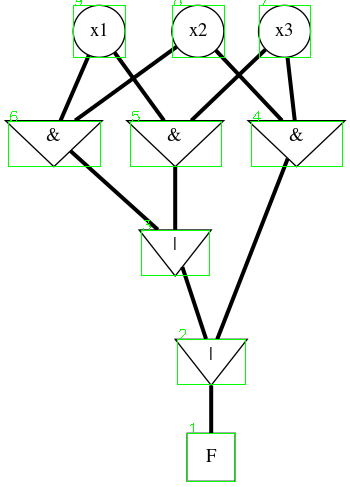
\includegraphics[scale=0.75]{img4_detected_vertices.png}
    \caption{Пример результата работы алгоритма выделения вершин СФЭ.}
\end{figure}

Выходом алгоритма сегментации является бинарное изображение с фигурами вершин.

\begin{figure}[H]
    \centering
    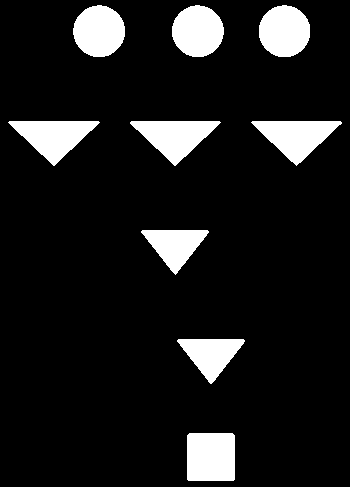
\includegraphics[scale=0.75]{img4_vertices.png}
    \caption{Пример выхода алгоритма сегментации СФЭ.}
\end{figure}


\subsection{Распознавание}
Этап распознавания разобьём на два подэтапа: распознавание меток в вершинах СФЭ и топологическое распознавание СФЭ.

\subsubsection{Распознавание меток}
Выходными данными алгоритма примененного на этапе сегментации является бинарное изображение с
фоновыми пикселями, имеющими значение $0$ и внутренностями вершин с контуром, имеющими значения $1$.
Таким образом, на самом деле, данное изображение является еще и маской для исходного изображения. А стало быть и для
его бинаризованного вида. Положим $M$ --- множество пикселей маски, а $B$ --- множество пикселей бинаризованного изображения.
Положим множество $L$ --- результат применения операцию конъюнкции к каждым пикселям ${{p_1}_i \in D}$ и ${{p_2}_i \in M}$,
то есть \[
    L = \{p_i \mid p_i = {p_1}_i \wedge {p_2}_i, {p_1}_i \in D, {p_2}_i \in M\}.
\]
$L$ --- бинарное изображение содержащее вершины и их метки заданной СФЭ.

\begin{figure}[H]
    \centering
    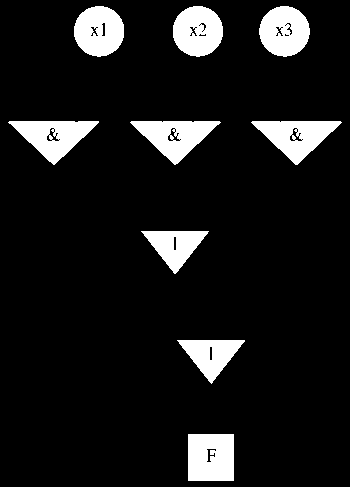
\includegraphics[scale=0.75]{img4_masked_vertices_labels.png}
    \caption{Пример изображения полученного в результате наложения маски на бинаризованное изображения содержащее СФЭ.}
\end{figure}

Далее, будем рассматривать каждую вершину по отдельности. Возьмем минимальный прямоугольник содержащий данную фиксированную вершину с меткой, обозначим
его через $r_1$. Такой прямоугольник содержит два класса пикселей: фоновые и полезные пиксели. Для удаления фоновых пикселей, инвертируем пиксели в
прямоугольнике содержащем множества пикселей вершин без метки, обозначим, такое множество за $r_2$. Применим попиксельно операцию дизъюнкции к $r_1$ и $r_2$. Получили множество пикселей, где фоновые пиксели имеют значение
$1$, а пиксели образующие метку --- значение $0$.

\begin{figure}[H]
    \centering
    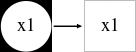
\includegraphics[scale=4]{label_detection.png}
    \caption{Пример результата работы алгоритма выделения метки.}
\end{figure}

Далее, к полученной изображению, применяя, к примеру, алгоритм распознавания текста основанный на нейронной сети с долгой краткосрочной памятью (в английской литературе LSTM based OCR) \cite{adnan16, tesseract}
получим текстовую запись метки данной вершины.

Таким образом, применяя приведенный алгоритм к каждой вершине СФЭ, получим все текстовые записи меток.

\subsubsection{Топологическое распознавание СФЭ}

\begin{definition}
    Ребром будем называть жорданову дугу образованную последовательностью точек ${p_i=1}$
    и соединяющее вершины ${v_i, v_j, i \neq j}$.
\end{definition}


Входными данными для топологического распознавания СФЭ является изображение полученное в результате дизъюнкции бинаризованное изображения СФЭ
с выходом алгоритма примененного на этапе сегментации --- бинарным изображением, содержащим исключительно вершины СФЭ.

\begin{figure}[H]
    \centering
    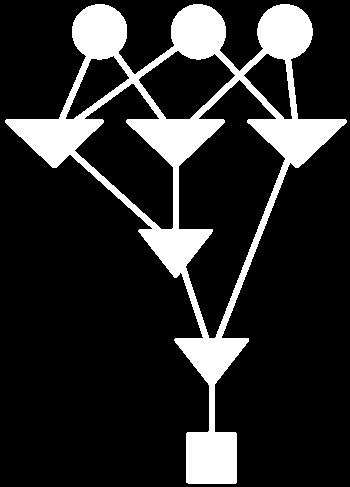
\includegraphics[scale=0.75]{img4_binarized_bfd.png}
    \caption{Пример входного изображения для алгоритма топологического распознавания СФЭ.}
    \label{fig:bfd}
\end{figure}

Алгоритм топологического распознавания СФЭ приведенный в данной работе основан на алгоритме топологического распознавания графа приведенного в работе \cite{auer13}.
Алгоритм топологического распознавания графа состоит из 3 частей: \emph{построение скелета графа}, \emph{классификация пикселей (точек) графа},
\emph{обход графа}. \\

\textbf{Рассмотрим процесс построение скелета графа.} Идея построения скелета объекта заключается в удалении пикселей из множества пикселей изучаемого объекта таким образом,
чтобы не нарушать топологию самого объекта. Результатом данной операции будет являться \emph{скелет} объекта.
Важным свойством процесса построения скелета объекта является сохранение свойства связности пикселей объекта. Это свойство
как раз и позволяет нам использовать данный процесс при топологическом распознавании графа.

Построение скелета графа основано на применении алгоритма предложенного в статье \cite{zhang_suen84}. Идея данного
алгоритма заключается в изменении значений пикселей с $1$ на $0$ контура объекта до тех пор, пока связность объекта не будет нарушена.

\begin{figure}[H]
    \centering
    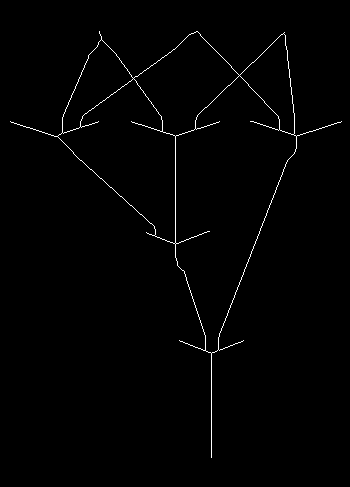
\includegraphics[scale=0.75]{img4_skelet.png}
    \caption{Пример результата работы построения скелета графа изображенного на рис. \ref{fig:bfd}.}
\end{figure}

\textbf{Рассмотрим процесс классификации пикселей графа.} Будем классифицировать каждый пиксель изображения как пиксель относящийся к одному из
следующих классов: $P_v$ --- класс пикселей входящих в одну из вершин графа (будем называть такой класс пикселей \emph{классом «порт» пикселей}),
$P_e$ --- класс пикселей представляющих собой пиксели одного из ребер графа, $P_c$ класс пикселей включающих в себя пиксели на пересечении двух ребер
(такой класс пикселей будем называть \emph{классом «кросс» пикселей}) и $P_b$ --- класс \emph{класс «фоновых» пикселей}, --- пиксели не входящие ни в один из приведенных ранее классов.

\begin{definition}
    Будем называть 4-окрестностью пикселя ${p_i}$ с координатами ${(x, y)}$ множество состоящее из пикселей с координатами
    ${(x-1, y), (x+1, y), (x, y-1), (x, y+1)}$.
\end{definition}

Напомним, что результатом построения скелета объекта изображенного на бинарном изображении является так же бинарным изображение.

Так как ранее, на этапе сегментации, мы однозначно выделили множество пикселей образующих вершины (с их внутренностью),
и скелет объекта включает так же данные пиксели (некоторое их подмножество), то мы можем однозначно отнести данные пиксели к классу $P_v$.

Пусть $P_r$ множество пикселей 4-окрестности пикселя $p_i$. \\
Положим \[
    n_0(p_i) = \sum_{p_j \in P_r} p_j.
\]

Будем считать, что пиксель $p_i$ относится к классу $P_b$, если $n_0(p_i) \le 1$, иначе если $n_0(p_i)=2$, то $p_i$ лежит в классе $P_e$,
иначе при $n_0(p_i) \ge 2$ пиксель лежит в классе $P_c$.

Таким образом, применяя изложенный алгоритм классификации к каждому пикселю получим 4 класса. При том, ни один из классов не содержит пиксели другого класса.

\begin{figure}[H]
    \centering
    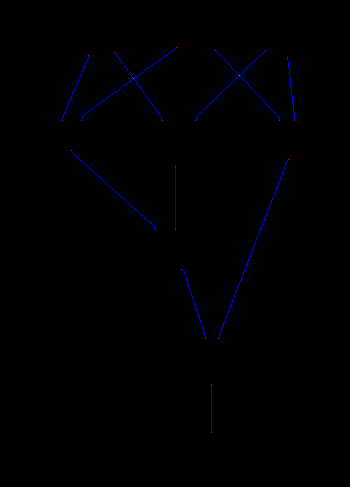
\includegraphics[scale=0.85]{img4_classified.png}
    \caption{Пример работы алгоритма классификации пикселей графа. Синим цветом выделены пиксели принадлежащие классу $P_e$, зеленым --- к классу $P_c$, красным --- к классу $P_v$, а черным --- к классу $P_b$.}
    \label{fig:img4_classified}
\end{figure}

Очевидно, что ребро всегда состоит из множества пикселей класса $P_e$, ``соединенное'' на концах с ровно одним пикселем из множества $P_v$. \\

\textbf{Рассмотрим процесс обхода графа.}
\begin{definition}
    Будем называть 8-окрестностью пикселя ${p}$ с координатами ${(x, y)}$ множество $N_8(p)$ состоящее из пикселей с координатами
    $\{(x-1, y-1), (x-1, y), (x-1, y+1), (x, y-1), (x, y+1), (x+1, y-1), (x+1, y), (x+1, y+1)\}$.
\end{definition}

Обход графа будем всегда начитать с пикселя принадлежащего классу $P_v$. Обход может быть осуществлен по всем пикселям за исключениям
пикселей принадлежащих классу $P_b$. Каждый уже пройденный пиксель будем помечать как пройденный.
Каждый следующий пиксель $p_{i+1} \in N_8(p_i)$ будем выбирать таким образом,
что выбранный пиксель $p_{i+1}$ не являлся бы ``пройденным''. \\

Тривиальным случаем является случай, когда ребро соединяющее две вершины $v_i$ и $v_j$ не пересекается ни с какими другими ребрами.
Для каждого такого тривиального случая будем считать, что между вершина $v_i$ и $v_j$, ${i \neq j}$ проведено ребро. \\

\emph{Направлением} будем называть вектор $\vec{v}=\overrightarrow{p_i,p_{i+1}}=(x_{i+1}-x_i, y_{i+1}-y_i)$.
\emph{Частотой} вектора $\vec{v}$ будем называть количество повторений вектора $\vec{v}$ в $n$ последних направлениях.
Обозначим последовательность $n$ последних направлений за $\{\vec{v_i}\}_{i=1}^{n}$.
Отметим, что последовательность $\{\vec{v_i}\}_{i=1}^{n}$, есть упорядоченная последовательность по частоте,
таким образом, что направления с большими частотами идут вначале.

Рассмотрим случай, когда ребро пересекает другое ребро в каком-то фиксированном пикселе $p_k \in P_c$.
Аналогично, обход графа начинаем с пикселя из класса $P_v$ и продолжаем ``идти'' по ребру, --- по пикселям класса $P_e$ до тех пор,
пока не ``встретим'' пиксель $p_k$. Если существует такой еще не ``пройденный'' пиксель $p_{i+1} \in N_8(p_k)$ и $p_{i+1} \in P_e \cup P_c$,
по одному из направлений $\vec{v_h} \in \{v_i\}_{i=1}^{n}$, то выберем данный пиксель $p_{i+1}$ как следующий пиксель за пикселем $p_i$;
иначе, если такого пикселя не существует, выберем пиксель $p_{i+1} \in N_8(p_k)$, такой что расстояние \[\rho(p_1, p_2) = \sqrt{\alpha(x_1-x_2)^2+\beta(y_1-y_2)^2}\]
от $p_i$ минимально. Здесь параметры $\alpha$ и $\beta$ определяются как средние количества изменений направления по осям $X$ и $Y$ соответственно.

Таким образом, применяя данный алгоритм для каждой вершины, то есть еще не пройденным пикселям $p_j \in P_v$ обойдем весь граф.

\subsection{Постобработка данных}
На данном этапе мы интерпретируем накопленные данные либо в текстовую форму записи формулы представленной СФЭ, либо в
код на языке программирования DOT. Для этого запустим алгоритм поиска в глубину \cite{dfs} от выходной вершины СФЭ и будем
интерпретировать вершины в зависимости от их значений. Отметим, что для бинарных операций (вершин с полустепенью захода $d(v) = 2$) последовательность входов будем считать по координате $x$ (относительно начала координат),
пикселей класса $P_v$ принадлежащих данной вершине и соединенных с пикселями $P_e$ каждого входящего ребра.

\section{Организация работы программы}
Программа для реализации алгоритма распознавания СФЭ приведенного в данной работе была написана на языке Python 3.
Для реализации промежуточных алгоритмов на стадиях бинаризации и сегментации была использована библиотека OpenCV 4 \cite{opencv4}.
Для реализации алгоритма распознавания символов была использована библиотека Tesseract 4 \cite{tesseract}. Для генерации кода на языке DOT для данной СФЭ
используется библиотека Graphviz.

Для интерпретации полученных данных была написана вспомогательная библиотека с реализацией структуры для построения Binary Expression Tree \cite{binary_tree},
и последующего его обхода, используя алгоритм поиска в глубину \cite{dfs} с применением шаблона проектирования «посетитель» (в английской литературе Visitor pattern) \cite{visitor}.
Таким образом, данная библиотека позволяет интерпретировать Binary Expression Tree построенное из полученных данных как в графическом представлении (то есть интерпретирует в цифровое изображение),
так и в текстовой записи.

\section{Результаты тестирования работы программы}
Для подтверждения эффективности алгоритма распознавания СФЭ предложенного в данной работе была составлена тестирующая программа. Данная программа случайным образом
генерировала СФЭ с различной сложностью, а именно: количество входных вершин случайным образом выбиралось в промежутке от 2 до 10, количество внутренних вершин
выбиралось как сумма количества входных вершин со случайным целым числом в промежутке от 0 до 10. Входы для внутренних вершин случайным образом выбирались либо из уже имеющихся входных и внутренних вершин, либо,
если количество входных вершин не превышало максимального допустимого количества (10) добавлялась новая входная вершина. Далее, полученная схема подавалась на вход программе реализующей распознавания СФЭ.
Выходом программы являлось так же графическое изображение СФЭ. Так как тестовое графическое изображение СФЭ и графическое изображение СФЭ полученное в результате распознавания генерировались одной и той программой, --- Graphviz,
то, если полученное графическое изображение СФЭ реализовывало ту же логическую формулу, что и тестовое графическое изображение СФЭ, оно должно быть идентично тестовому графическому изображению СФЭ (входному).
Стало быть, для проверки корректности полученного изображения СФЭ достаточно попиксельно сравнить его с исходным изображением. \\
Тестовые испытания проводились на данных размерами $20$, $30$ и $50$. При том, каждый тест запускался 3 раза. Так для тестового массива данных с размерностью $20$ вероятность корректно распознавания СФЭ составила $\frac{14}{20}$,
с размерностью $30$ --- $\frac{64}{90}$, с размерность $50$ --- $\frac{115}{150}$.
Так было полученное, что СФЭ без самопересечений распознается с вероятностью $1$, для СФЭ с самопересечениями вероятность составила $0.6$. \\

\newpage

Приведем изображения некоторых успешно распознанных СФЭ.

\begin{figure}[H]
    \centering
    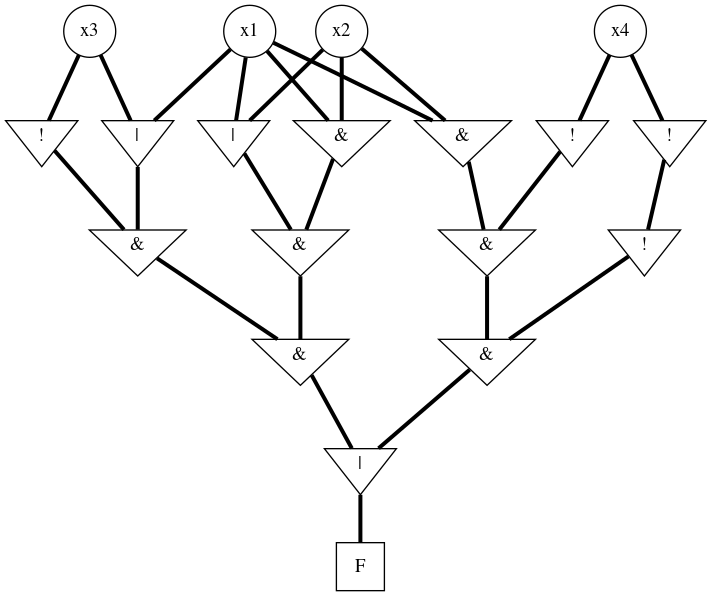
\includegraphics[scale=0.45]{example1.png}
\end{figure}

\begin{figure}[H]
    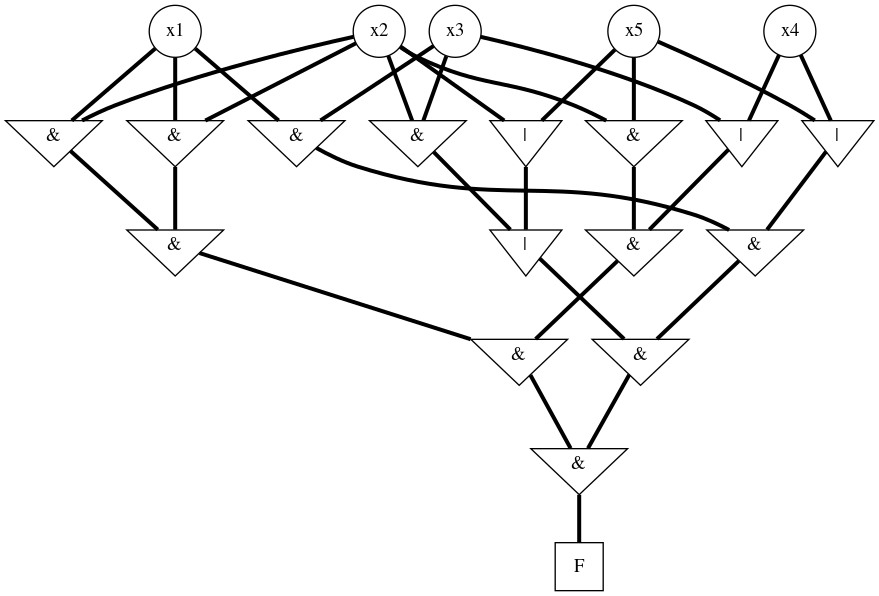
\includegraphics[scale=0.5]{example4.png}
\end{figure}

\begin{figure}[H]
    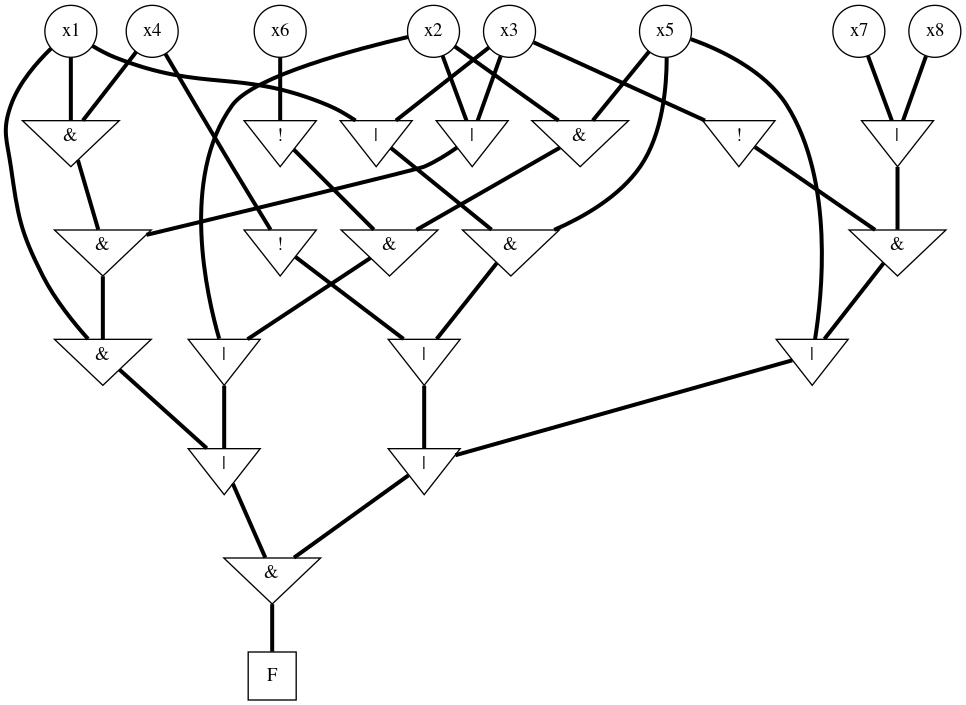
\includegraphics[scale=0.4]{example6.png}
\end{figure}

\begin{figure}[H]
    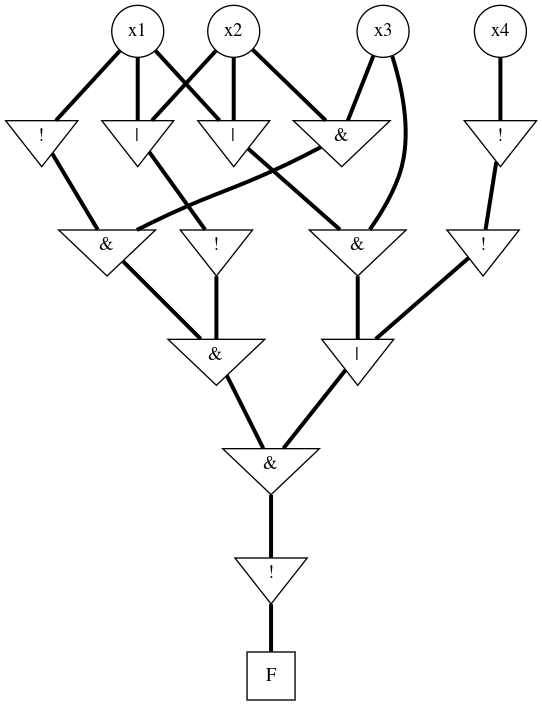
\includegraphics[scale=0.45]{example3.png}
    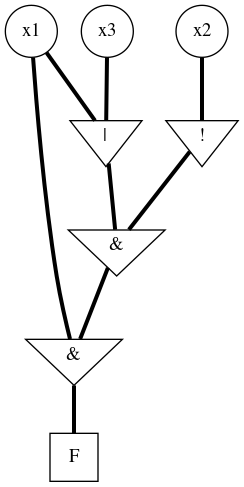
\includegraphics[scale=0.65]{example2.png}
\end{figure}

Рассмотрим некоторые пример СФЭ, для которых система распознавания СФЭ выдала некорректный результат. \\

Проблему для топологического распознавания СФЭ составляют случаи с пересечениями ребер как, например, на рисунке \ref{fig:bad_recognition}.

\begin{figure}[H]
    \centering
    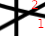
\includegraphics[scale=5.5]{bad_recognition.png}
    \caption{Пример пересечения ребер ведущих к некорректному распознаванию СФЭ.}
    \label{fig:bad_recognition}
\end{figure}

В процессе построения скелета СФЭ, два участка ``1'' и ``2'' различных ребер ``сливаются'' в один контур на участке ``3'' как изображено на рисунке \ref{fig:bad_recognition_skelet}.

\begin{figure}[H]
    \centering
    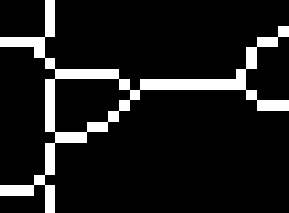
\includegraphics[scale=1]{bad_recognition_skelet.png}
    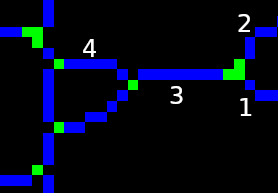
\includegraphics[scale=1.1]{bad_recognition_classified.png}
    \caption{Пример части скелета СФЭ ведущих к некорректному распознаванию СФЭ.}
    \label{fig:bad_recognition_skelet}
\end{figure}

Это ведет к тому, что при прохождении участка ``3'' и при достаточно малом $n$ (напомним, что это параметр, который указывает на максимальную длину последовательности последних $n$ векторов направления,
использующийся в алгоритме топологического распознавания графа.), частота вектора направления $\vec{v}=(-1, 0)$, будет максимальной,
что приведет к тому, что для обоих участков ``1'' и ``2'' двух различных ребер продолжением будет считаться один и тот же участок ``4''.

Одним из способов решения данной проблемы является выбор $n$, таким, что частота вектора направления $\vec{v}=(-1, 0)$ не будет максимальной.
Однако, экспериментальным путем было выявлено, что $n=4$, является оптимальным для большего количества задач. \\

Рассмотрим следующую проблему, --- проблему корректной сегментации СФЭ.

\begin{figure}[H]
    \centering
    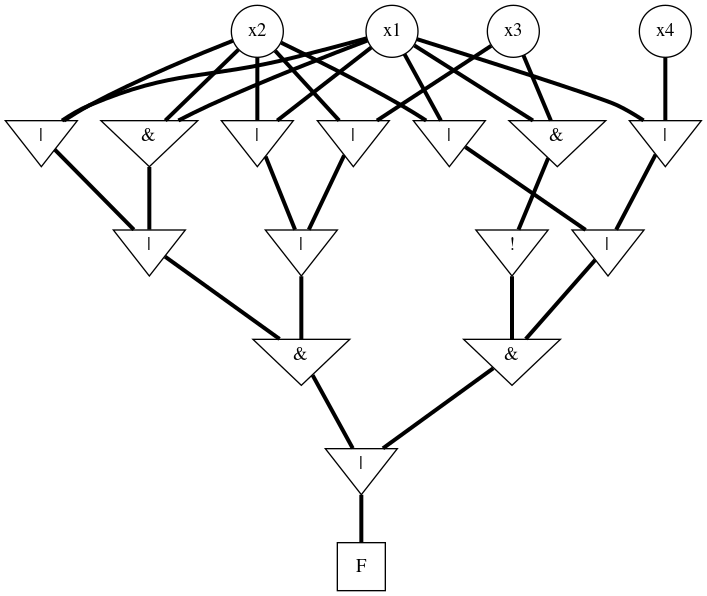
\includegraphics[scale=0.4]{bad_segmentation.png}
    \caption{Пример СФЭ порождающей проблему сегментации (корректного выделения вершин) СФЭ.}
    \label{fig:bad_segmentation}
\end{figure}

На рисунке \ref{fig:bad_segmentation} приведено изображение СФЭ, которое влечет проблему сегментации.
На рисунке \ref{fig:bad_segmentation_nodes} приведен результат алгоритма детекции вершин примененного к изображению СФЭ на рисунке \ref{fig:bad_segmentation}.

\begin{figure}[H]
    \centering
    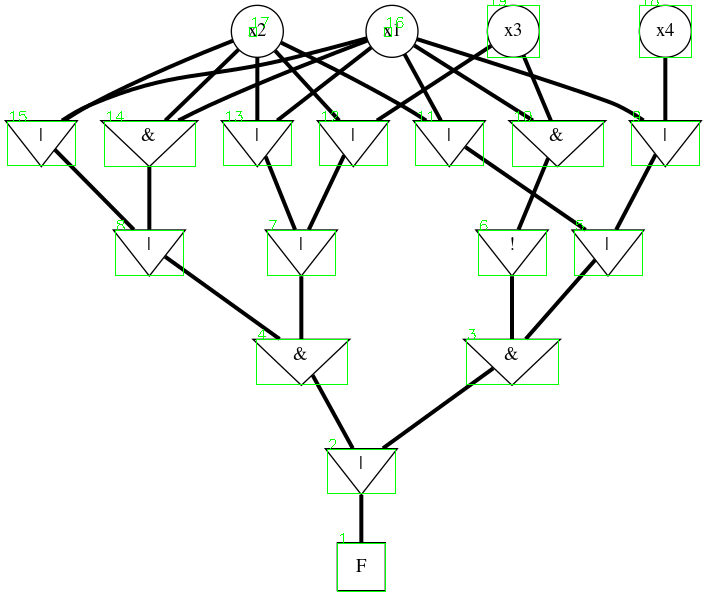
\includegraphics[scale=0.5]{bad_segmentation_nodes.png}
    \caption{Пример СФЭ порождающей проблему сегментации (корректного выделения вершин) СФЭ.}
    \label{fig:bad_segmentation_nodes}
\end{figure}

Как можно видеть, вершины с метками ``x2'' и ``x1'' не были выделены. Это произошло по причине того,
что вокруг них имеется превалирующее количество фигур образованных пересечением ребер. Так как в алгоритме выделения вершины для каждой фигуры
проверяются все 3 условия, то при проверке условия 3 (об отсутствии пересечений минимальных описывающих прямоугольников с другими
минимальным описывающими прямоугольниками) для вершин с метками ``x2'' и ``x1'' их минимальные описывающие прямоугольники будут пересекаться с описывающими прямоугольниками фигур, образованных пересечением ребер и при том
площади данных вершин будут большими. Таким образом вершины с метками ``x2'' и ``x1'' будут исключены из множества вершин.

Одним из способов коррекции данного поведения, является пропуск проверки условия 3 для вершин.
Однако, такое решение может повлечь проблемы при детекции вершин в других задача распознавания СФЭ. \\

Помимо проведения тестирования на задача сгенерированных программой для тестирования, так же были проведены испытания
на СФЭ нарисованных от руки.

Рассмотрим первый пример графического изображения СФЭ нарисованного от руки.

\begin{figure}[H]
    \centering
    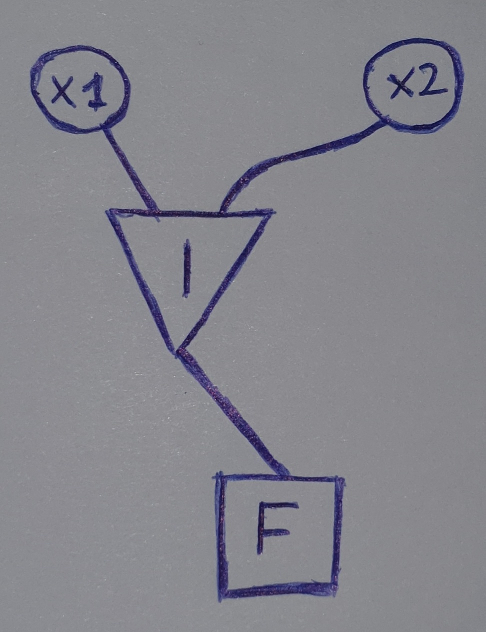
\includegraphics[width=60mm]{handwritten_2.png}
    \caption{Пример графического изображения СФЭ нарисованного от руки.}
    \label{fig:handwritten_2}
\end{figure}

\begin{figure}[H]
    \centering
    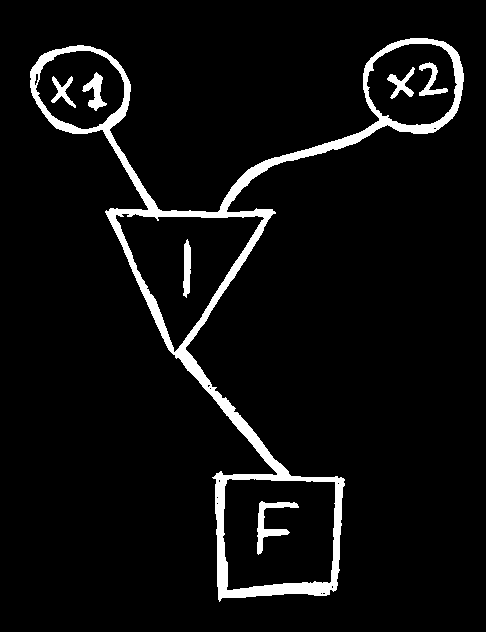
\includegraphics[width=55mm]{handwritten_2_binarized_image.png}
    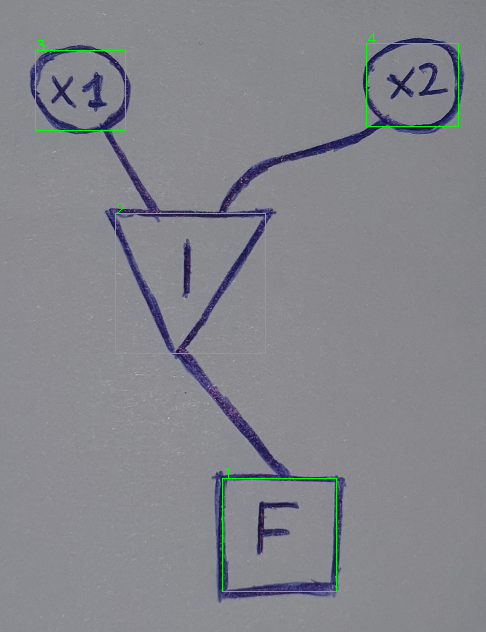
\includegraphics[width=55mm]{handwritten_2_detect_labels.png}
    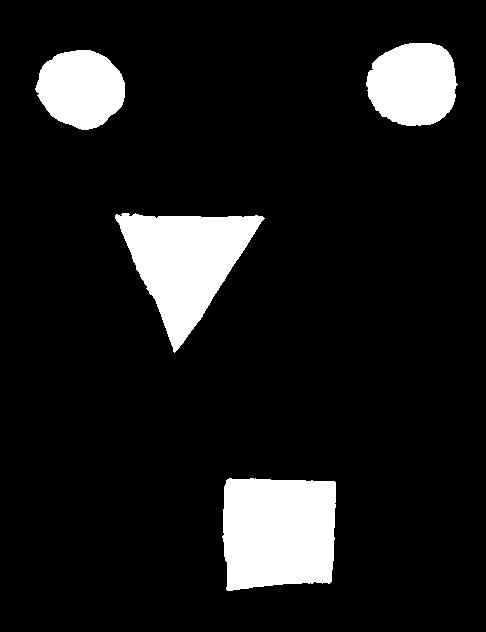
\includegraphics[width=55mm]{handwritten_2_vertices_pixels.png}
    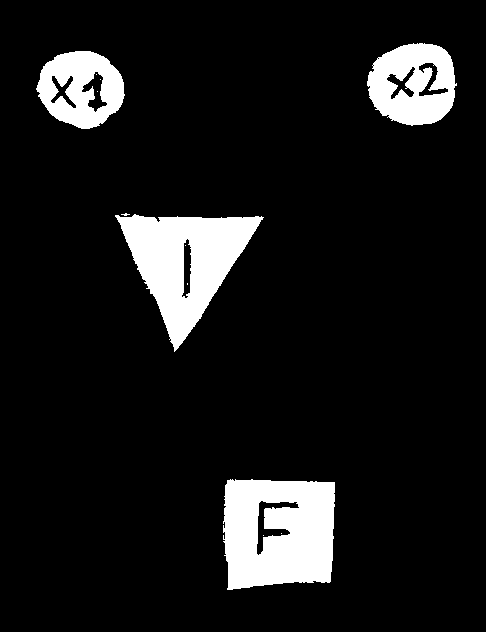
\includegraphics[width=55mm]{handwritten_2_masked.png}
    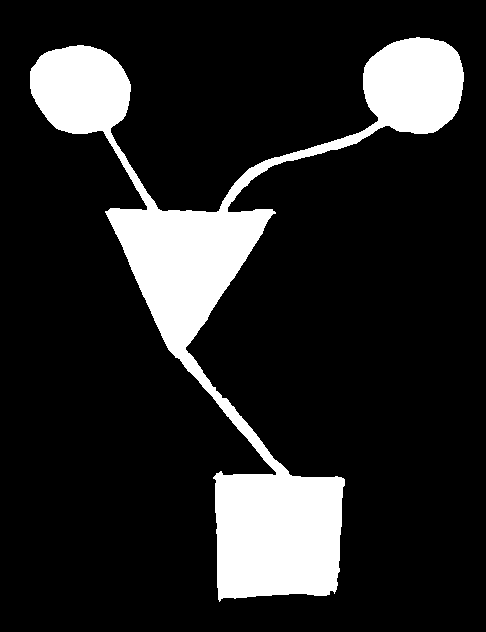
\includegraphics[width=55mm]{handwritten_2_processed_image.png}
    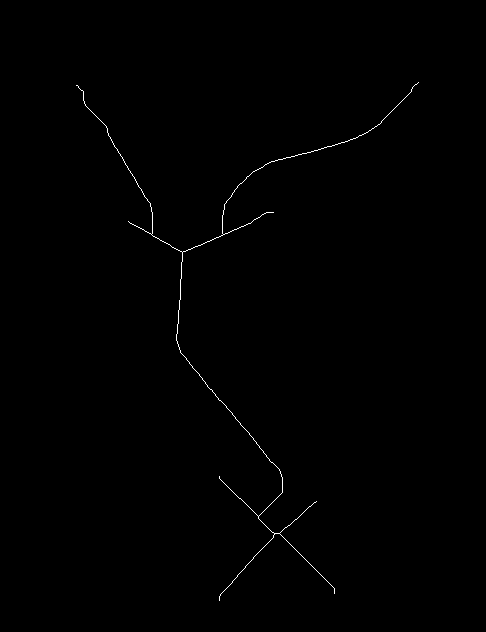
\includegraphics[width=55mm]{handwritten_2_image_skelet.png}
\end{figure}

\begin{figure}[H]
        \centering
        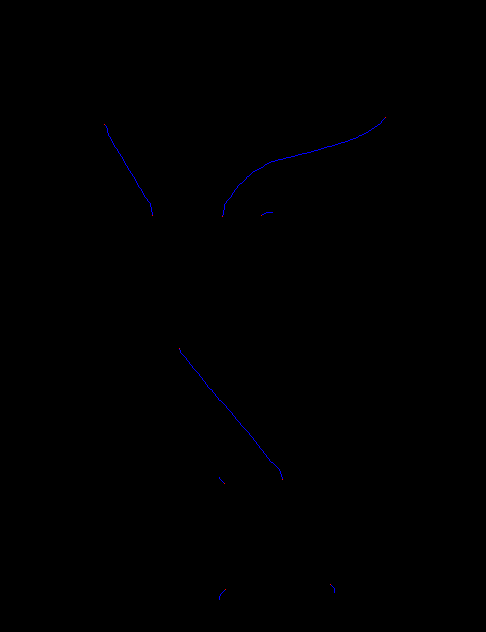
\includegraphics[width=55mm]{handwritten_2_classified_pixels.png}
\end{figure}

\begin{figure}[H]
    \centering
    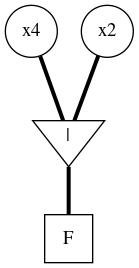
\includegraphics{handwritten_2_result.png}
    \caption{Результат распознавания СФЭ изображенной на рис. \ref{fig:handwritten_2}}
\end{figure}

\newpage

Рассмотрим второй пример графического изображения СФЭ нарисованного от руки.

\begin{figure}[H]
    \centering
    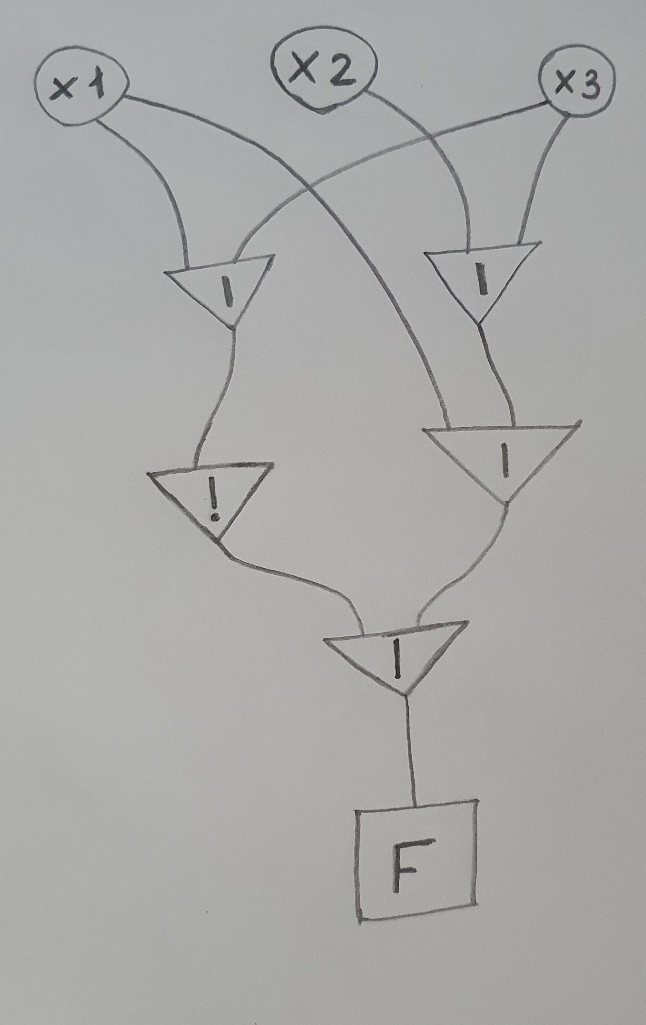
\includegraphics[width=55mm]{handwritten_1.png}
    \caption{Пример графического изображения СФЭ нарисованного от руки.}
    \label{fig:handwritten_1}
\end{figure}


\begin{figure}[H]
    \centering
    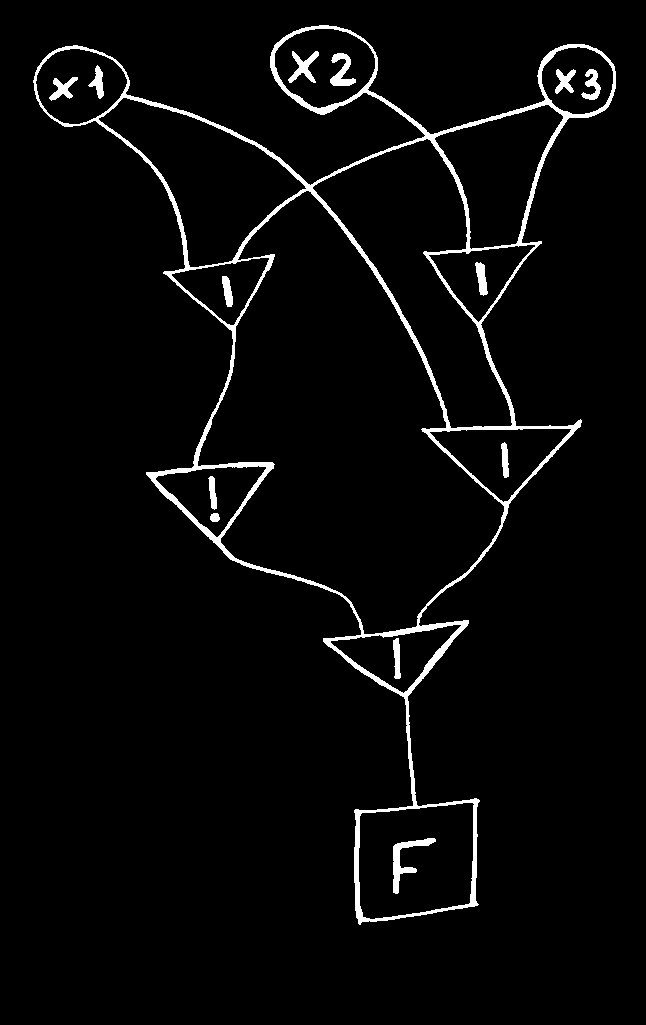
\includegraphics[width=70mm]{handwritten_1_binarized_image.png}
    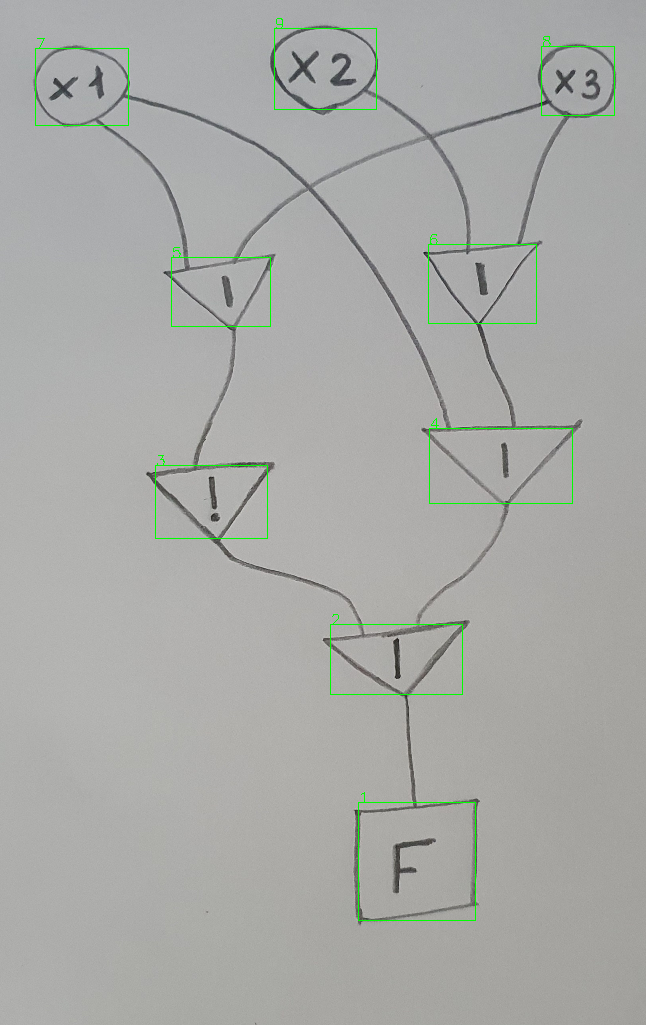
\includegraphics[width=70mm]{handwritten_1_detect_labels.png}
\end{figure}

\begin{figure}[H]
    \centering
    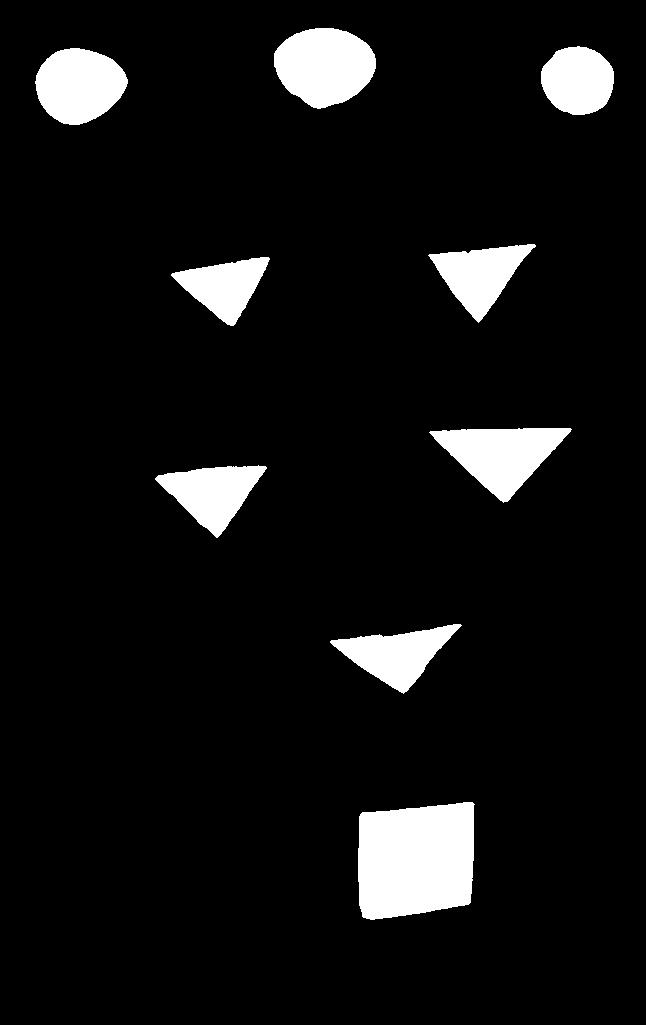
\includegraphics[width=70mm]{handwritten_1_vertices_pixels.png}
    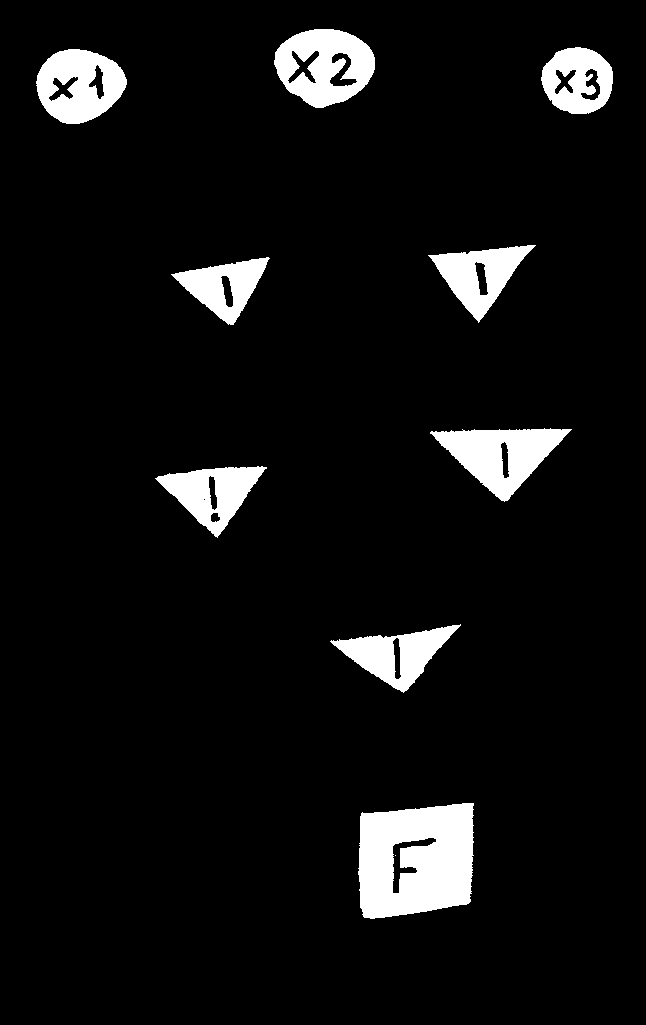
\includegraphics[width=70mm]{handwritten_1_masked.png}
    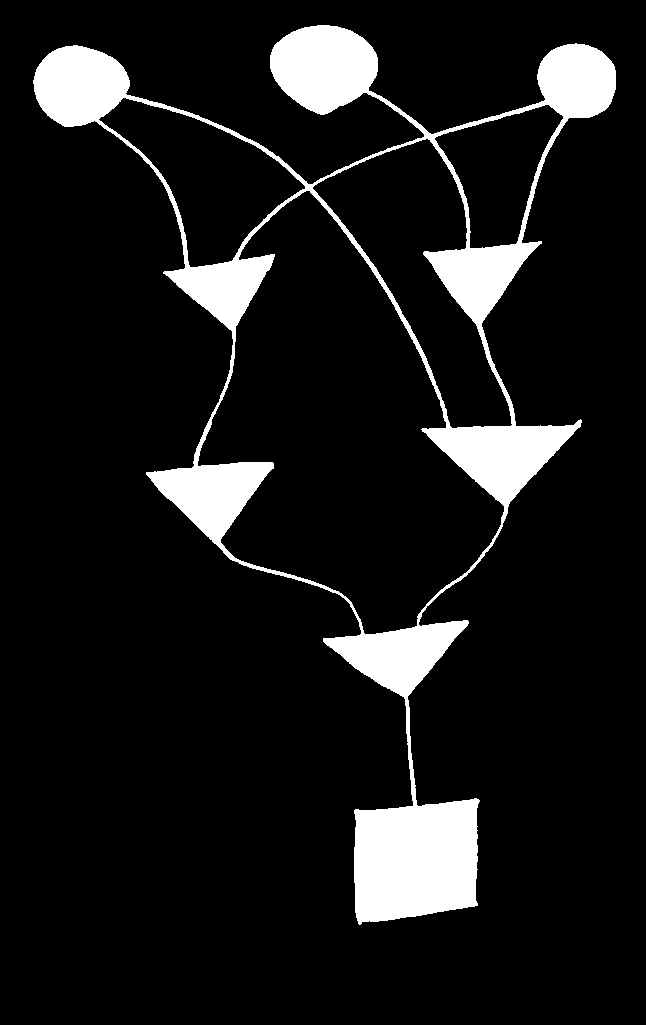
\includegraphics[width=70mm]{handwritten_1_processed_image.png}
    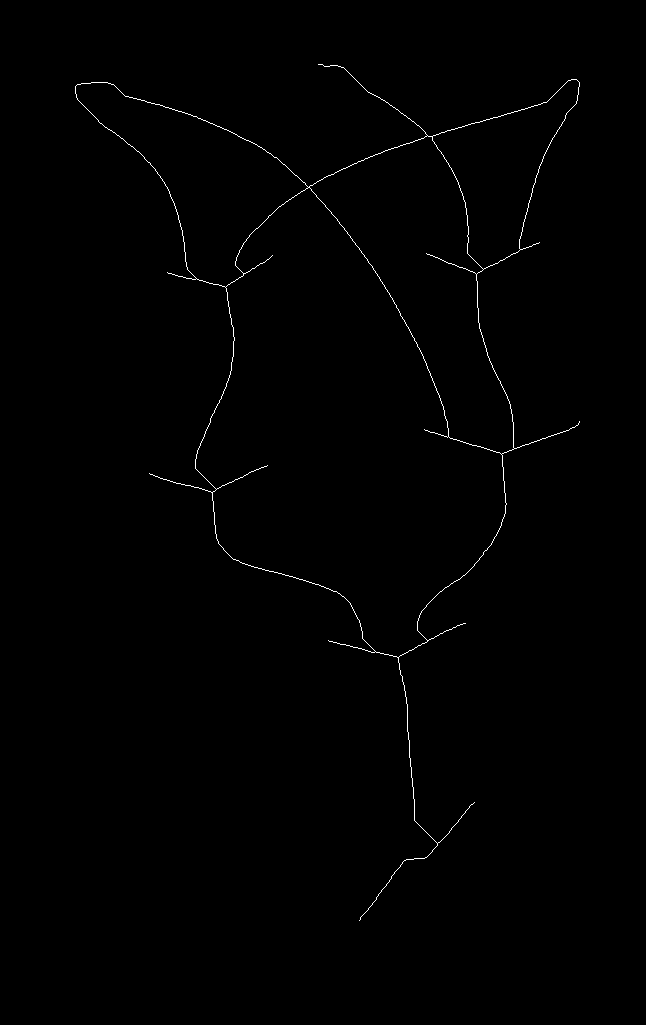
\includegraphics[width=70mm]{handwritten_1_image_skelet.png}
\end{figure}

\begin{figure}[H]
    \centering
    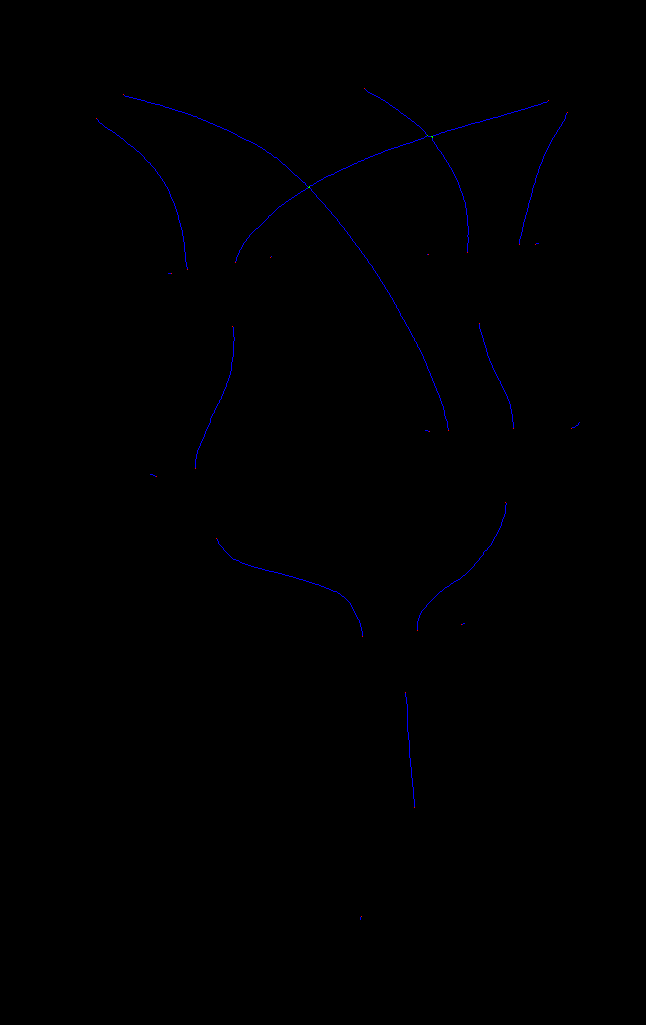
\includegraphics[width=70mm]{handwritten_1_classified_pixels.png}
\end{figure}

\begin{figure}[H]
    \centering
    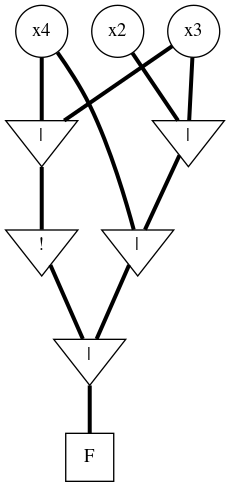
\includegraphics[width=50mm]{handwritten_1_result.png}
    \caption{Результат распознавания СФЭ изображенной на рис. \ref{fig:handwritten_1}}
\end{figure}

Как можно видеть, топология обеих СФЭ была распознана корректно. В обоих случаях все вершины были распознаны так же корректно, за исключением вершин с меткой ``x1'', они были распознаны как ``x4''.
Это связано с тем, что в прототипе программы для распознавания СФЭ для задачи распознавания меток использовалась библиотека Tesseract со стандартной обученной моделью.
Данная модель ``хорошо'' работает для задачи распознавания текста (слов), но не столь хорошо для посимвольного распознавания.
Если дообучить данную модель на ``нужных'' нам данных (символах), то проблему некорректного распознавания меток можно разрешить.

\section{Заключение}
В рамках данной работы был предложен и реализован алгоритм для распознавания схем из функциональных элементов.
Для упрощения изложения рассматривались схемы из функциональных элементов заданные над стандартным базисом ${B = \{x_1 \wedge x_2, x_1 \vee x_2, \neg{x_1}\}}$.
Оптическое распознавание СФЭ осуществлялось в 4 этапа: предварительная обработка данных, сегментация, распознавание и постобработка данных.
Результаты полученные при тестировании работы программы вполне подтверждают применимость данного подхода для задачи распознавания СФЭ.
Так было полученное, что СФЭ без самопересечений распознается с вероятностью $1$, а для СФЭ с самопересечениями вероятность составила $0.6$.
Были рассмотрены некоторые изображения СФЭ, которые распознавались некорректно и предложены решения для коррекции проблем возникших для данных классов задач.

\begin{thebibliography}{}
    \bibitem{dot_lang} \url{https://en.wikipedia.org/wiki/DOT_(graph_description_language)}
    \bibitem{graphviz}
        \url{https://www.graphviz.org/}
    \bibitem{grayscale_luma} \url{https://en.wikipedia.org/wiki/Luma_(video)#Rec._601_luma_versus_Rec._709_luma_coefficients}
    \bibitem{otsu79} N. Otsu.
        \textit{A threshold selection method from gray-level histograms. IEEE Trans. Sys., Man., Cyber. : journal. — 1979. — Vol. 9. — P. 62—66.}
    \bibitem{suzuki85} Suzuki, S. and Abe, K.,
        \textit{Topological Structural Analysis of Digitized Binary Images by Border Following. CVGIP 30 1, pp 32-46 (1985)}
    \bibitem{adnan16} Adnan Ul-Hasan
        \textit{Generic Text Recognition using Long Short-Term Memory Networks}
        \url{https://kluedo.ub.uni-kl.de/frontdoor/deliver/index/docId/4353/file/PhD_Thesis_Ul-Hasan.pdf}
    \bibitem{tesseract}
        \url{https://tesseract-ocr.github.io/}
    \bibitem{auer13} Ch. Auer, Ch. Bachmaier, F. Gleißner, and J. Reislhuber
        \textit{Optical Graph Recognition, section 3.3, p. 6-9.}
        \url{https://link.springer.com/content/pdf/10.1007%2F978-3-642-36763-2_47.pdf}
    \bibitem{zhang_suen84}  T. Y. Zhang, C.Y. Suen
        \textit{A Fast parallel algorithm for thinning digital petterns.}
        \url{http://agcggs680.pbworks.com/f/Zhan-Suen_algorithm.pdf}
    \bibitem{opencv4}
        \url{https://opencv.org/opencv-4-0/}
    \bibitem{binary_tree}
        \url{https://en.wikipedia.org/wiki/Binary_expression_tree}
    \bibitem{dfs}
        \url{https://en.wikipedia.org/wiki/Tree_traversal#Depth-first_search}
    \bibitem{visitor}
        \url{https://en.wikipedia.org/wiki/Visitor_pattern}
\end{thebibliography}

\end{document}
